\documentclass[12pt,draftcls,onecolumn]{IEEEtran}
\usepackage{amsmath,amssymb}
\usepackage{graphicx}
\usepackage{booktabs}
\usepackage{cite}
\usepackage{url}
\usepackage[hidelinks]{hyperref}

\newtheorem{proposition}{Proposition}
\newtheorem{corollary}{Corollary}
\newtheorem{definition}{Definition}

\begin{document}

\title{Competing Platforms in Mobile Crowdsensing:\\ An Agent-Based Study of Learning Platforms and Strategic Users}

\author{Abdullah Sajid (27100144) and Mishal Sagar (27100166)\\
EE567/CS6315 Multiagent Systems, Lahore University of Management Sciences\\
Code and data: \texttt{\url{https://github.com/abdullahsajidfr/competing-platforms-crowdsensing}}}

\maketitle

\begin{abstract}
Mobile crowdsensing apps pay smartphone users to collect data such as air quality or traffic, and several apps often compete for the same users. Recent learning-based mechanisms let an app learn rivals' prices from reports by users who reject it, assuming these reports are truthful. We study what happens when that assumption fails, and how learning apps price and cover a city. We model each hour as a leader--follower game: apps post budget-limited bounties on 500\,m cells, and users choose at most one task and share a cell's bounty with co-workers. We prove that the users' game is an exact potential game, so a pure Nash equilibrium exists and best-response play reaches it, and that truthful reporting is not incentive compatible under rival-offer learning. We also compute Nash and joint-profit benchmarks for the apps' pricing game. A Mesa simulation replays one real week of Beijing T-Drive taxi and GeoLife pedestrian traces for 300 users. Results show that users reach an equilibrium every hour, within 2\% of a greedy planner's welfare on average. When half the users inflate reports, reporting and non-reporting cohorts both earn more on average, and app profit falls 7--12\%. With two apps, Q-learning settles below Nash pay without demonstrable collusion, and a 50\% bonus raises low-traffic coverage 18-fold at equal budget. Ablations show that price and budget dominate outcomes. Next steps are to test a faithful PACMAB implementation, adaptive reporting, and defences against false reports.
\end{abstract}

% ======================================================================
\section{Introduction and Literature Review}
\subsection{Motivation}
Mobile crowdsensing (MCS) replaces fixed sensor networks with people. Platforms post sensing tasks, such as a noise reading or an air-quality sample. Smartphone users who pass nearby perform the tasks for payment. The approach is cheap and covers the city wherever people go. It has been used for traffic, environmental monitoring and market research~\cite{li2021mp}.

Most incentive-design work assumes one platform~\cite{yang2012crowdsourcing}. In practice, several apps compete for the same finite pool of users. Each user can do only one task at a time, so the apps must outbid each other~\cite{li2021mp,dongare2026pacmab}.

Competition raises three questions that single-platform models cannot answer:
\begin{enumerate}
\item \emph{Strategic reporting.} An app does not see its rivals' prices. The state-of-the-art multi-platform learner, PACMAB~\cite{dongare2026pacmab}, therefore learns them from \emph{users' reports}: a user who rejects an app tells it which rival offer they took and at what pay. PACMAB assumes these reports are truthful. A self-interested user, however, may exaggerate the rival offer to get better offers later.
\item \emph{Learned prices.} Apps increasingly set prices with learning algorithms. In product markets, independent Q-learning sellers learn supracompetitive prices without communicating~\cite{calvano2020ai}. For apps that \emph{buy} data, the analogous risk is that learning holds user pay down.
\item \emph{Spatial coverage.} Users go where routes and bounties take them. Low-traffic areas may stay uncovered whatever the apps pay.
\end{enumerate}

Our research questions follow directly:
\begin{itemize}
\item \textbf{RQ1:} Do false rival offers raise users' net earnings or platform spending?
\item \textbf{RQ2:} Do learning platforms raise or lower payments over time?
\item \textbf{RQ3:} Are low-traffic areas left uncovered, and can a bonus help?
\item \textbf{RQ4:} Which pricing method gives the best coverage per unit budget?
\end{itemize}

The papers below are the ones the model is built on. For each we give the problem it addresses, its relevance to our setup, what we took from it, and its key findings.

\subsection{Incentive mechanisms for a single platform}
\textbf{Yang et al.~\cite{yang2012crowdsourcing}.}
\emph{Problem:} how one platform should pay smartphone users to sense. In the platform-centric model the platform announces a total reward $R$, each user chooses a sensing time $t_i$, and user $i$ receives $R\,t_i/\sum_k t_k$ at cost $t_i\kappa_i$. In the user-centric model, users bid in a reverse auction (MSensing).
\emph{Relevance:} this is the template for our game. The platform is a Stackelberg leader and users are followers who share a reward. Our equal split of a cell's bounty is the discrete counterpart of their proportional split, and we keep their notation $\kappa_i$ for a user's private cost.
\emph{Insight:} the leader's problem is solved by backward induction. First compute the users' equilibrium for each reward, then optimise the reward against it. Our platform price matrix does this numerically.
\emph{Key findings:} the platform-centric game has a unique Stackelberg equilibrium that can be computed efficiently. MSensing is computationally efficient, individually rational, profitable and truthful.

\subsection{Multiple competing platforms}
\textbf{Li et al., MP-Coopetition~\cite{li2021mp}.}
\emph{Problem:} incentive design when several platforms compete or cooperate. Competing platforms price rewards to attract participants and users choose which platform to work for; this is modelled as a two-stage Stackelberg game. Cooperating platforms share data through many-to-many bargaining.
\emph{Relevance:} it is the closest prior model to ours: several leaders and a population of followers who choose a platform.
\emph{Insight:} the equilibrium notion is Nash competition among the leaders, with users best-responding underneath. Our model differs in three ways: platforms learn their prices, users may misreport, and users move on real routes, so coverage is an outcome.
\emph{Key findings:} competing platforms secure their payoff by pricing rewards optimally, and users pick the best platform. Exact bargaining is NP-hard, so a heuristic is proposed; cooperation further raises platform payoffs.

\textbf{Dongare et al., PACMAB~\cite{dongare2026pacmab}.}
\emph{Problem:} task assignment when several platforms send personalised task offers to the same users. Platforms do not know rivals' preferences or users' qualities, and users do not know task efforts. The interaction is a matching game with contracts, posed as a dynamic hypergame in which each platform holds perceptions of its rivals and refines them over time.
\emph{Relevance:} PACMAB is the mechanism our RQ1 examines, and the source of two modelling choices. Each user performs at most one task per time step, and a user who rejects a platform tells it which rival task was accepted and at what payment. PACMAB assumes this feedback is truthful, and its perception update keeps the maximum reported rival payment.
\emph{Insight:} rival prices are learned from users' reports, which cost nothing to falsify. Under a max-based update, a single inflated report raises the estimate permanently. Our rival-offer learning is a simplified per-cell version of this rule, and we also test the max update.
\emph{Key findings:} platforms run combinatorial UCB bandits over payment levels and users run bandits over task efforts. The scheme is fully decentralised and reaches a hyper Nash equilibrium given the perceptions. It completes at least 41\% more tasks than the benchmarks, with 99.8\% task completion.

\subsection{Congestion and potential games}
\textbf{Rosenthal~\cite{rosenthal1973}.}
\emph{Problem:} which games always have a pure Nash equilibrium.
\emph{Key finding:} in a congestion game, players choose resources and a resource's payoff depends only on how many use it. Every such game has a pure NE, a maximiser of $\sum_e\sum_{\ell=1}^{n_e}r_e(\ell)$.
\emph{Relevance and insight:} each (platform, cell) pair in our model is a resource whose per-user payoff $R_{jg}/n_{jg}$ falls with its load. Rosenthal's function gives our potential directly (Proposition~\ref{prop:potential}).

\textbf{Monderer and Shapley~\cite{monderer1996potential}.}
\emph{Problem:} games in which every unilateral change in a player's payoff equals the change in one global function.
\emph{Key findings:} every finite potential game has the finite improvement property: any sequence of strict unilateral improvements ends at a pure NE. Congestion games are potential games, and every finite potential game is isomorphic to a congestion game.
\emph{Relevance and insight:} this is why best response in our simulator stops at an equilibrium every hour. We check it numerically by confirming that the potential never decreases.

\textbf{Blume~\cite{blume1993}; Marden and Shamma~\cite{marden2012revisiting}.}
\emph{Problem:} which equilibrium boundedly rational players select.
\emph{Key findings:} under log-linear learning, a revising player picks action $x$ with probability proportional to $e^{u(x)/T}$. In potential games the stationary distribution is proportional to $e^{\Phi/T}$, so as $T\to0$ play concentrates on potential maximisers. Marden and Shamma show this survives asynchronous or simultaneous revision, restricted action sets and payoff-based implementations.
\emph{Relevance and insight:} our user game has many equilibria, and log-linear learning gives a principled way to select among them. In our pilot, lower temperatures reached higher-potential equilibria.

\textbf{Vetta~\cite{vetta2002}.}
\emph{Problem:} how much welfare selfish play loses in valid utility games, where the social objective is submodular and each player receives at least its marginal contribution.
\emph{Key finding:} every NE achieves at least half the optimal welfare (price of anarchy at most 2), with applications including facility location.
\emph{Relevance and insight:} our platforms' cell value $q(n)=1-(1-\rho)^n$ is submodular, as in sensor placement. But our users receive equal shares, not their marginal contribution, so the bound is not guaranteed. We therefore measure efficiency numerically.

\subsection{Learning and algorithmic pricing}
\textbf{Watkins and Dayan~\cite{watkins1992}.}
\emph{Problem:} learning optimal decisions in an unknown Markov decision process from experience.
\emph{Key finding:} the update $Q(s,a)\leftarrow(1-\alpha)Q(s,a)+\alpha[r+\gamma\max_{a'}Q(s',a')]$ converges to the optimal values with probability 1 if the environment is stationary, every state--action pair is visited infinitely often, and step sizes decay suitably.
\emph{Relevance and insight:} our platforms use this update over price levels. With several learners each one's environment is non-stationary, so the guarantee does not hold, and we check convergence empirically.

\textbf{Calvano et al.~\cite{calvano2020ai}.}
\emph{Problem:} whether independent Q-learning sellers in a repeated Bertrand oligopoly learn to collude without communicating.
\emph{Relevance:} RQ2 asks the same question of platforms that buy data. For buyers, collusion means pay held below the competitive level.
\emph{Insight:} we follow their experimental design: a price grid around the Nash and joint-profit prices, one-period memory as the state, decaying exploration, a stability-based convergence rule, the profit-gain index $\Delta=(\bar\Pi-\Pi^N)/(\Pi^C-\Pi^N)$, and control runs that remove the ability to punish or to value the future.
\emph{Key findings:} the algorithms learn supracompetitive prices, typically with $\Delta$ of 70--90\%. These prices are sustained by punishing deviations, followed by a gradual return to high prices, and collusion weakens with more firms. High (here, low) prices alone do not prove collusion.

\subsection{Data and simulation tools}
CrowdSenSim~\cite{fiandrino2017crowdsensim} simulates crowdsensing in realistic urban environments and shows the importance of realistic mobility, which is why we replay real traces. T-Drive~\cite{yuan2010tdrive} gives one week of GPS traces from 10,357 Beijing taxis. GeoLife~\cite{zheng2010geolife} gives 2007--2012 trajectories of 182 users, mostly in Beijing. Mesa~\cite{kazil2020mesa} is the Python agent-based modelling framework the simulator is built on.

\subsection{Our approach}
Li et al.~\cite{li2021mp} solve for equilibrium prices with fully rational platforms. PACMAB~\cite{dongare2026pacmab} learns prices under truthful user feedback. We combine learning platforms whose price estimates come from possibly false user reports, a potential-game analysis of the users' side, and a simulation on real city-scale mobility. This lets us measure who gains from misreporting, whether learned pay is competitive, and where coverage fails.

% ======================================================================
\section{Problem Setup: Game-Theoretic Formulation}\label{sec:model}
\subsection{Environment}
\begin{itemize}
\item \emph{Space.} Central Beijing is divided into $|\mathcal G|=1368$ cells of 500\,m ($36\times38$).
\item \emph{Time.} A round $t$ represents one hour, with hour-of-week index $\tau\in\{0,\dots,167\}$. In chronological replays, $\tau(t)=t\bmod168$.
\item \emph{Routes.} In round $t$, user $i$'s trace passes through cells $P_i(t)$; if $P_i(t)=\emptyset$, the user is inactive. The user can reach cells $\mathcal G_i(t)$, namely the route plus its 4-neighbours. The detour is $d_i(g)=0$ on the route and $0.5$\,km otherwise.
\item \emph{Low-traffic cells.} $L\subset\mathcal G$ is the 25\% of cells that users pass near least often.
\end{itemize}

\subsection{Players}
\begin{itemize}
\item \textbf{Platforms} $j\in\mathcal J=\{1,\dots,M\}$, $M\in\{2,3,4\}$: air quality, traffic, noise and weather. Each platform has:
  \begin{itemize}
  \item cell weights $w_{jg}\in[0,1]$, giving how much it values cell $g$;
  \item a value $V$ for a fully covered weight-1 cell;
  \item an hourly budget $B_j$.
  \end{itemize}
\item \textbf{Users} $i\in\mathcal N$, $|\mathcal N|=300$. User $i$'s private type is $\theta_i=(c_i,\kappa_i,h_i,\beta_i,\delta_i)$:
  \begin{itemize}
  \item $c_i$: per-task cost;
  \item $\kappa_i$: detour cost per km;
  \item $h_i$, $\beta_i$: home app and loyalty bonus (loyal users only);
  \item $\delta_i$: report inflation ($\delta_i=0$ for honest users).
  \end{itemize}
\end{itemize}

\subsection{Stage game played every hour (leader--follower)}
\textbf{Stage 1: platforms act (leaders).}
\begin{itemize}
\item Platform $j$ chooses candidate bounties $\tilde R_{jg}(t)$ through its pricing rule (Section~\ref{sec:rules}).
\item It posts tasks on reachable cells in decreasing order of $w_{jg}$, as long as the total posted bounty stays within $B_j$. Call the posted set $S_j(t)$; set $R_{jg}=\tilde R_{jg}$ for $g\in S_j(t)$.
\item Because a platform pays at most the posted bounty per cell, spending never exceeds $B_j$.
\end{itemize}

\textbf{Stage 2: users act (followers).}
\begin{itemize}
\item User $i$ chooses
\[a_i\in A_i(t)=\{(j,g): g\in\mathcal G_i(t)\cap S_j(t)\}\cup\{\varnothing\},\]
i.e.\ at most one task per hour, following~\cite{dongare2026pacmab}.
\item The load is $n_{jg}(a)=|\{i:a_i=(j,g)\}|$, and co-workers split the bounty equally.
\end{itemize}

\textbf{Utilities.}
\begin{align}
u_i(a)&=\begin{cases}\dfrac{R_{jg}}{n_{jg}(a)}-c_i-\kappa_i d_i(g)+\beta_i\mathbf 1[j=h_i], & a_i=(j,g),\\[4pt] 0, & a_i=\varnothing,\end{cases}\label{eq:user}\\
\pi_j(a)&=\sum_g w_{jg}V\,q\big(n_{jg}(a)\big)-\sum_g R_{jg}\mathbf 1[n_{jg}(a)\ge1],\qquad q(n)=1-(1-\rho)^n.\label{eq:platform}
\end{align}
Here $q(n)$ is the probability that at least one of $n$ readings is usable. It is increasing and concave, so the value of a cell has diminishing returns (it is submodular).

\textbf{Welfare.} Payments are transfers between players, so social welfare is
\[W(a)=\sum_j\sum_g w_{jg}Vq(n_{jg})-\sum_{i:a_i\ne\varnothing}\big(c_i+\kappa_id_i(a_i)\big).\]

\textbf{Reports.} A user working for $k$ at cell $g$ earns $x_i=R_{kg}/n_{kg}$. They send every rejected platform $j\neq k$ the report
\[r_{i\to j}=(1+\delta_i)\,x_i.\]
Reports never change the payment already agreed.

\subsection{Pricing (decision update) rules}\label{sec:rules}
\begin{enumerate}
\item \textbf{Fixed price (baseline).} $\tilde R_{jg}=m\,w_{jg}\,b$, with a constant price level $m$ and base reward $b$.
\item \textbf{Q-learning.} $\tilde R_{jg}(t)=m_j(t)w_{jg}b$, with $m_j(t)$ chosen from a grid $\mathcal M$.
  \begin{itemize}
  \item State: $s_t=(m_1,\dots,m_M)(t-1)$.
  \item Action: $\varepsilon$-greedy over $Q_j(s_t,\cdot)$, with $\varepsilon_t=e^{-\beta_\varepsilon t}$.
  \item Update: $Q_j(s,m)\leftarrow(1-\alpha)Q_j(s,m)+\alpha\,[\pi_j+\gamma\max_{m'}Q_j(s',m')]$, with $\alpha=0.15$ and $\gamma=0.95$~\cite{calvano2020ai}.
  \end{itemize}
\item \textbf{Rival-offer learning} (simplified PACMAB). For each cell, platform $j$ keeps an estimate $\hat o_{jg}$ of the best rival per-person pay.
  \begin{itemize}
  \item After receiving reports, let $r_{jg}^{\max}=\max_i r_{i\to j,g}$. The first observed maximum initialises $\hat o_{jg}$. Later reports update it by
  \[\hat o_{jg}\leftarrow(1-\eta)\hat o_{jg}+\eta r_{jg}^{\max},\qquad
    \text{or}\qquad \hat o_{jg}\leftarrow\max\{\hat o_{jg},r_{jg}^{\max}\}.\]
  Then set $\tilde R_{jg}\leftarrow\min(\hat o_{jg}+\lambda,\,w_{jg}V\rho)$: outbid, but never pay more than one reading is worth.
  \item After winning a cell with no reports: $\tilde R_{jg}\leftarrow\max((1-\zeta)\tilde R_{jg},\,0.2w_{jg}b)$, a slow price cut.
  \item After an unfilled task: $\tilde R_{jg}\leftarrow\min((1+\zeta)\tilde R_{jg},\,w_{jg}V\rho)$, a slow price rise.
  \end{itemize}
\item \textbf{Users' rule.} Asynchronous best response from the empty profile: a random-order sweep in which each user switches to a strictly better action, repeated until no one moves. We also study best response with inertia and log-linear learning.
\end{enumerate}

\subsection{Equilibrium analysis for the baseline}\label{sec:eq}
\begin{proposition}[Users' game is a potential game]\label{prop:potential}
For any posted bounties $R$, the users' game is an exact potential game with
\[\Phi(a)=\sum_{(j,g)}\sum_{\ell=1}^{n_{jg}(a)}\frac{R_{jg}}{\ell}-\sum_{i:a_i\neq\varnothing}\Big(c_i+\kappa_id_i(a_i)-\beta_i\mathbf 1[j(a_i)=h_i]\Big).\]
\end{proposition}
\begin{IEEEproof}
Fix $a_{-i}$, and let user $i$ move from $e=(j,g)$ to $e'=(j',g')$.
\begin{itemize}
\item The load on $e$ drops from $n_e$ to $n_e-1$, so the first sum loses its last term $R_e/n_e$.
\item The load on $e'$ rises from $n_{e'}$ to $n_{e'}+1$, so the first sum gains $R_{e'}/(n_{e'}+1)$.
\item In the second sum, only user $i$'s own term changes.
\end{itemize}
Hence
\[\Phi(e',a_{-i})-\Phi(e,a_{-i})=\frac{R_{e'}}{n_{e'}+1}-\frac{R_e}{n_e}-\big[c_i+\kappa_id_i(g')-\beta_i\mathbf 1[j'=h_i]\big]+\big[c_i+\kappa_id_i(g)-\beta_i\mathbf 1[j=h_i]\big],\]
which equals $u_i(e',a_{-i})-u_i(e,a_{-i})$ by~\eqref{eq:user}. Moves to or from $\varnothing$ are identical, with one of the two load terms absent.
\end{IEEEproof}

\begin{corollary}\label{cor:ne}
(i) A pure NE exists: any maximiser of $\Phi$ over the finite action space.
(ii) Every sequence of strict unilateral improvements is finite~\cite{monderer1996potential}, so asynchronous best response terminates at a pure NE. Best response with inertia converges almost surely.
(iii) Under log-linear learning, the stationary distribution is $\propto e^{\Phi/T}$~\cite{blume1993}.
(iv) In any NE, every active participant has $u_i\ge0$ (individual rationality), since $\varnothing$ is always available.
\end{corollary}

\textbf{Multiplicity and selection.} Equilibria are generally not unique. In 300 random small instances (4 users, 3 cells, 2 platforms), solved by brute force, there were on average 6.05 pure NE per instance (maximum 24). We therefore fix the selection rule: asynchronous best response from the empty profile with a fixed seed.

\begin{proposition}[Coverage threshold]\label{prop:cov}
Fix the posted tasks and bounties, and let $e=(j,g)$ be a posted task. For a user $i$ who can reach $e$, let $U_i^{-e}$ be the maximum of zero and the utilities $R_{j'g'}-c_i-\kappa_id_i(g')+\beta_i\mathbf 1[j'=h_i]$ from taking another feasible posted task $(j',g')\ne e$ alone. If $a^\ast$ is a NE with $n_{jg}(a^\ast)=0$, then every such user satisfies
\[R_{jg}\le u_i(a^\ast)+c_i+\kappa_id_i(g)-\beta_i\mathbf 1[j=h_i].\]
In particular, $e$ is covered in every NE if some eligible user $i$ satisfies
\[R_{jg}>U_i^{-e}+c_i+\kappa_id_i(g)-\beta_i\mathbf 1[j=h_i].\]
\end{proposition}
\begin{IEEEproof}
If $e$ is empty, a deviation to it yields the full bounty less the user's costs, plus any loyalty bonus. At a NE this cannot exceed $u_i(a^\ast)$, giving the first inequality. When $e$ is empty, $i$ is either inactive or on another feasible task whose payoff is bounded above by its solo payoff. Thus $u_i(a^\ast)\le U_i^{-e}$ in any NE leaving $e$ empty. The sufficient condition would contradict this, and its right-hand side depends on the posted alternatives, not on the selected NE.
\end{IEEEproof}

\emph{Toy example.} With one platform, two posted tasks A and B with positive bounties, and two users who can reach both at zero cost, $(A,A)$ is a NE exactly when $R_B\le R_A/2$. A split is a NE exactly when $R_A/2\le R_B\le2R_A$, and $(B,B)$ is a NE exactly when $R_B\ge2R_A$. Thus B is covered in every NE exactly when $R_B>R_A/2$. At equality, $(A,A)$ and $(A,B)$ are both equilibria.

Proposition~\ref{prop:cov} helps explain RQ3: a reachable user may prefer a busy cell unless the low-traffic task offsets their opportunity and detour costs. A uniform increase of $m$ can raise the payoff of competing tasks too, so it need not close the gap. If changing a bounty changes which tasks are posted, the condition must be evaluated for the resulting menu.

\textbf{Efficiency.} The welfare $W$ is a submodular coverage function. But users receive equal shares rather than their marginal contribution, so Vetta's price-of-anarchy bound of 2~\cite{vetta2002} is not guaranteed. In the 300 small instances, the brute-force PoA averaged 1.22 (worst 2.81) and the PoS averaged 1.08. On real data, we compare the NE against a greedy planner in Section~\ref{sec:setup}.

\textbf{Platforms' price game and the Stackelberg view.} Fix the users' response $a^\ast(R(m))$ selected above. The platforms then play a simultaneous game
\[\Gamma^P=(\mathcal J,\mathcal M^M,\Pi),\qquad \Pi_j(m)=\tfrac1{168}\sum_{\tau=0}^{167}\pi_j\big(a^\ast_\tau(R(m))\big),\]
where the average runs over the 168 real hours for one seed (seed 0). A NE of $\Gamma^P$ together with $a^\ast$ is a subgame-perfect equilibrium of the benchmark in which platforms commit to prices before the hour is drawn and users respond after observing it. It need not be a Nash price profile for each individual hour. We compute $\Pi$ exhaustively on the grid $\mathcal M=\{0.4,0.6,\dots,1.6\}$ for $M=2$ (Fig.~\ref{fig:price}).
\begin{itemize}
\item \emph{No pure NE exists.} The best responses form an Edgeworth-type cycle: each platform outbids the other, until undercutting becomes more profitable.
\item \emph{The unique mixed NE} was found by support enumeration. Platform 1 plays $\{0.8\!:\!0.06,\ 1.0\!:\!0.94\}$; platform 2 plays $\{0.6\!:\!0.74,\ 0.8\!:\!0.26\}$. Expected price levels are $(0.99,0.65)$, mean 0.82, and joint profit is $\Pi^N=451.5$.
\item \emph{The joint-profit (``collusive'') profile} is $(0.8,0.6)$, with $\Pi^C=491.5$.
\end{itemize}
Platforms buy data, so collusion would suppress pay. We measure learned outcomes with $\Delta=(\bar\Pi-\Pi^N)/(\Pi^C-\Pi^N)$, where $\bar\Pi$, $\Pi^N$ and $\Pi^C$ are all \emph{joint} hourly profit (the sum across platforms), whereas $\Pi_j(m)$ is platform $j$'s hourly profit. Calvano et al.~\cite{calvano2020ai} use per-firm average profit; for a fixed number of firms, dividing each joint total by $M$ leaves the ratio unchanged, in particular in the symmetric case. For $M=3,4$ there is also no pure NE, and we do not compute a mixed NE. We substitute the myopic learners' joint profit for $\Pi^N$ in $\Delta$ for those cases.

\begin{figure}[!htbp]\centering
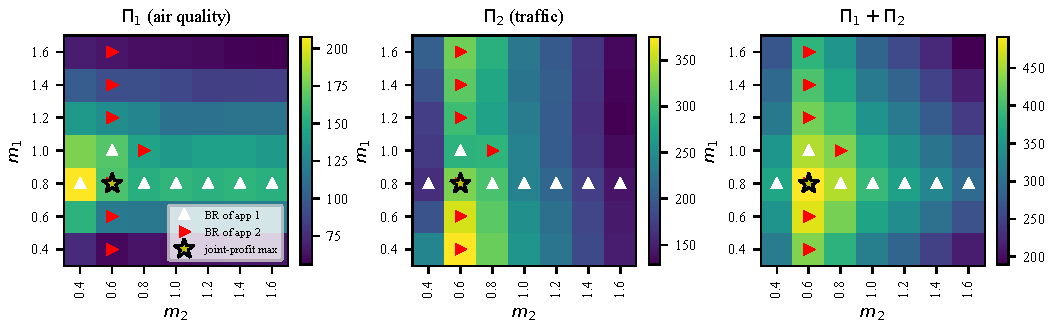
\includegraphics[width=\linewidth]{figs/price_game.pdf}
\caption{Platforms' price game for $M=2$ on real traces (seed 0; profit per price profile averaged over 168 hours). Markers show each platform's best response to the rival's price and the joint-profit maximum. The best responses never intersect, so there is no pure NE.}
\label{fig:price}
\end{figure}

\begin{proposition}[Truthful reporting is not incentive compatible in repeated play]\label{prop:ic}
In the one-shot reporting stage, all reports are payoff-equivalent and every report is a best response. Under either rival-offer update, truthful reporting need not be a best response in repeated play, so the mechanism is not incentive compatible in general.
\end{proposition}
\begin{IEEEproof}
\emph{One-shot game.} Reporting follows the task choice and does not change the agreed payment. Holding the task choices fixed, no report strictly improves current utility over any other, so none weakly dominates another under the definition requiring a strict gain for some opponents' actions.

\emph{Repeated game.} Consider two rounds, one on-route user with cost 1 and no loyalty bonus, and two platforms posting on the same cell. Let $b=5$, $V=20$, $\rho=0.5$ and $m=1$ initially. With weights 0.6 and 0.4 the first-round bounties are 3 and 2. The user takes the first offer. The rejected platform starts with no estimate and uses the first observed report to initialise it under either update. With $\lambda=0.25$ and a cap of 4, a truthful report of 3 makes its next bounty 3.25, while a 50\% inflated report makes it 4. The first platform, having won the user without a report, cuts its bounty to 2.94 ($\zeta=0.02$). With slack budgets and the same cell reachable in both rounds, the user takes the second platform's offer in round two under either report, gaining 0.75 from inflation. Any positive weight on the second-round payoff therefore makes the deviation profitable.
\end{IEEEproof}
A higher candidate bounty does not guarantee a higher payoff: with a binding budget it can crowd other tasks out of $S_j$, including a task the reporting user would have taken. Conversely, when a higher bounty is posted, honest users can also benefit from it. Whether spending rises and how the gains are shared are empirical questions (RQ1).

% ======================================================================
\section{Simulation Setup and Results}\label{sec:setup}
\subsection{Setup}
\begin{itemize}
\item \emph{Data processing.} T-Drive fixes are interpolated every 100\,m, and GPS jumps above 120\,km/h are removed. GeoLife hours count as walking if the median speed is at most 6\,km/h; they are overlaid on the T-Drive week by weekday and hour.
\item \emph{Implementation.} The Mesa model coordinates user and platform agents. Settings use 10 seeds unless noted; Mesa seeds change costs and types, not routes. Truthful and lying runs share routes, costs and seeds. The 25\% strategic-user set is a subset of the 50\% set, so we compare the same people.
\item \emph{Q-learning horizon.} Training repeatedly samples hours uniformly from the precomputed 168-hour payoff bank rather than replaying the hours in order. A run stops once exploration is below 0.01 and the greedy policy has stayed unchanged for 25,000 rounds, or at the round cap. Downstream evaluation of the learned policies replays the trace week twice.
\item \emph{Parameters.} Table~\ref{tab:params}.
\end{itemize}

\begin{table}[!htbp]\centering
\caption{Simulation parameters (baseline in bold).}\label{tab:params}
\begin{tabular}{@{}ll@{}}\toprule
Cells / users & 1368 cells of 500\,m; 200 taxis + 100 pedestrians (121 active per hour on average, range 16--232)\\
Costs & $c_i\sim U[1,3]$; $\kappa_i\sim U[0.5,2]$ (taxis), $U[1,4]$ (pedestrians) per km\\
Platforms & $M\in\{\mathbf 2,3,4\}$; $b=5$, $V=20$, $\rho=0.5$; weights from observed taxi/pedestrian activity\\
Budget per platform & $B\in\{150,\mathbf{300},600\}$ per hour\\
Users' types & 20\% loyal ($\beta=1$); 0 / 25 / 50\% strategic ($\delta=0.5$, also 1.0)\\
Baseline pricing & fixed price, $\mathbf{m=1}$\\
Q-learning & $\alpha=0.15$, $\gamma=0.95$, $\varepsilon_t=e^{-10^{-5}t}$, up to $1.5\times10^6$ rounds\\
Rival-offer & $\eta=0.2$, $\lambda=0.25$, $\zeta=0.02$\\
Fixed-price runs & 10 seeds; 2 replay weeks \\
Rival-offer runs & 10 seeds; 5 replay weeks, first 2 discarded as burn-in \\
\bottomrule\end{tabular}
\end{table}

\begin{figure}[!htbp]\centering
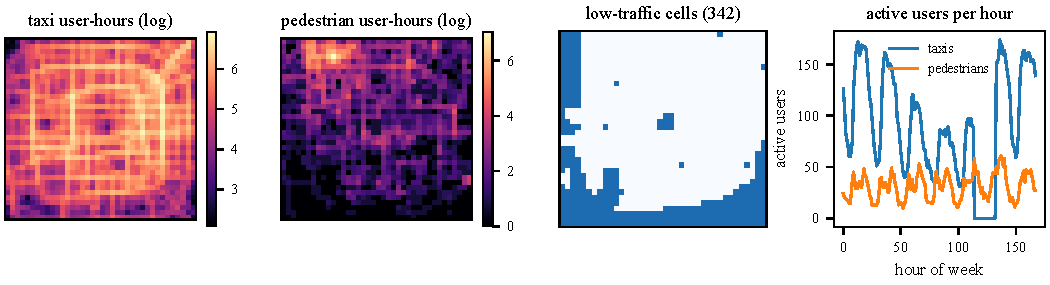
\includegraphics[width=\linewidth]{figs/data.pdf}
\caption{Real Beijing traces on the 500\,m grid: taxi and pedestrian activity, low-traffic cells, and active users per hour. The gap around hour 115 is missing T-Drive data during the Spring Festival.}
\label{fig:data}
\end{figure}

\subsection{Baseline results and link to the equilibrium analysis}
The baseline uses a fixed price $m=1$, $M=2$, $B=300$ and 20\% loyal users. Users settle by best response.

\textbf{Equilibrium reached every hour (Corollary~\ref{cor:ne}).}
\begin{itemize}
\item We tested every alternative action of every active user, in all 168 hours: no user could gain by switching.
\item Best response needed 3.3 sweeps on average (maximum 6).
\item The potential rose monotonically and flattened at the equilibrium (Fig.~\ref{fig:eq}a--b).
\end{itemize}

\textbf{Efficiency.} Using the same posted tasks, a greedy planner adds the (user, task) pair with the largest marginal welfare gain until none is positive.
\begin{itemize}
\item The equilibrium's welfare averaged 98.9\% of the greedy planner's ($M=2$), 99.4\% ($M=3$) and 98.1\% ($M=4$), with a worst hour of 91.8\% (Fig.~\ref{fig:eq}c).
\item In about 30\% of hours (9\% for $M=4$), the equilibrium even beat the greedy planner.
\end{itemize}
So, although Vetta's bound is not guaranteed under equal sharing, selfish task choice is nearly efficient on real mobility. The large worst-case PoA found in the toy instances does not show up here.

\begin{figure}[!htbp]\centering
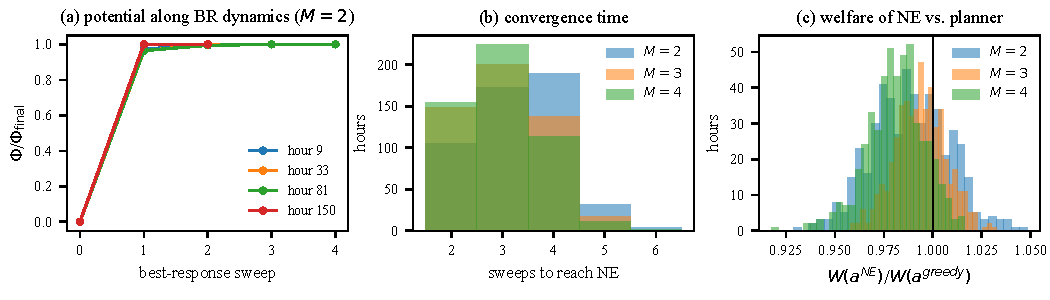
\includegraphics[width=\linewidth]{figs/equilibrium.pdf}
\caption{Equilibrium diagnostics on real data. (a) The potential $\Phi$ rises monotonically under best response (Proposition~\ref{prop:potential}). (b) Sweeps needed to reach a NE, over 504 hours per $M$. (c) Welfare of the reached NE relative to a greedy planner.}
\label{fig:eq}
\end{figure}

\textbf{Outcomes.}
\begin{itemize}
\item 79.8 of 1368 cells are covered per hour.
\item Across both platforms, mean hourly payouts are 352 and mean hourly profit (sensing value minus payouts) is 377.
\item 71\% of active users participate and 55\% of posted tasks are completed.
\item Users earn a net 1.40 per active hour; the Gini coefficient of earnings is 0.37.
\item Only \textbf{0.74 of the 342 low-traffic cells} are covered per hour, consistent with Proposition~\ref{prop:cov}.
\end{itemize}

\subsection{Ablation studies}
Fig.~\ref{fig:abl} varies one parameter at a time around the baseline (10 seeds each).

\begin{figure}[!htbp]\centering
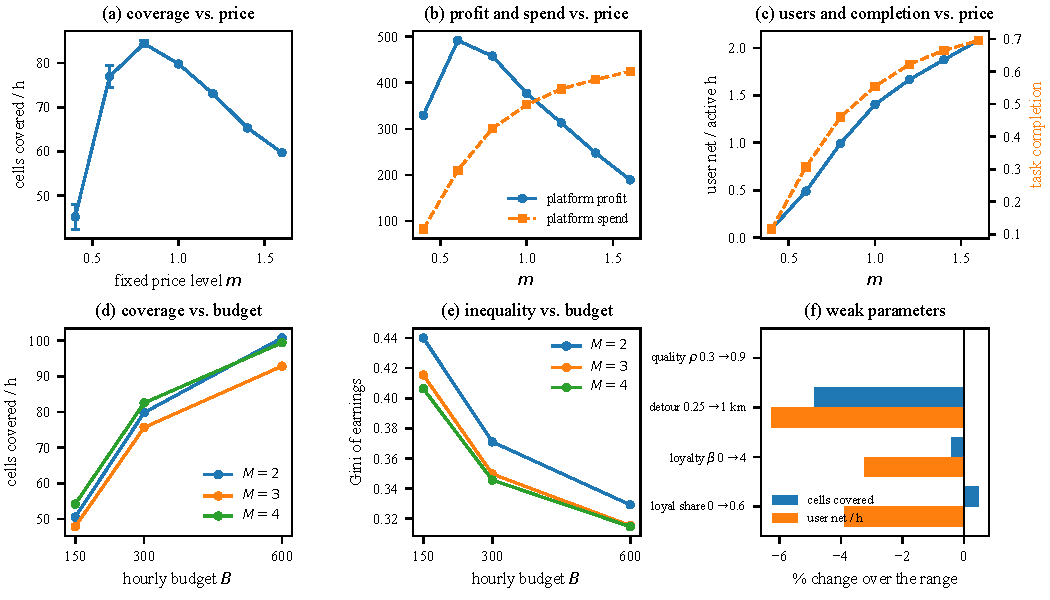
\includegraphics[width=\linewidth]{figs/ablations.pdf}
\caption{Baseline ablations (fixed price, $M=2$, $B=300$ unless varied; 10 seeds). (a--c) Price level $m$. (d--e) Budget and number of platforms. (f) Change in coverage and user earnings over the full range of each weak parameter.}
\label{fig:abl}
\end{figure}

\begin{enumerate}
\item \textbf{Price level $m$: an interior optimum, caused by the budget.}
  \begin{itemize}
  \item Coverage rises from 45 cells ($m=0.4$) to a peak of 84 ($m=0.8$), then falls to 60 ($m=1.6$).
  \item Joint profit peaks at a common $m=0.6$ (491.76 per hour) and falls to 189 at $m=1.6$.
  \item User earnings and task completion rise monotonically: 0.09 to 2.08 per active hour, and 12\% to 70\% completion.
  \end{itemize}
  \emph{Insight.} Below $m\approx0.8$, few users meet the participation condition (Corollary~\ref{cor:ne}(iv)). Above it, the binding budget posts fewer, pricier tasks, so higher pay buys \emph{less} coverage. The ablation varies a common $m$ and averages 10 seeds over two weeks. The price game allows each platform to choose its own $m_j$ and averages one seed over 168 hours. Within that same price-game benchmark, joint profit is 476.98 at $(0.6,0.6)$ versus 491.47 at the maximiser $(0.8,0.6)$.
\item \textbf{Budget $B$ and number of platforms $M$.}
  \begin{itemize}
  \item Doubling the budget from 150 to 300 to 600 raises coverage from 51 to 80 to 101 cells ($M=2$).
  \item Participation rises from 49\% to 86\%, and the Gini falls from 0.44 to 0.33, because more users find a task worth taking.
  \item Task completion falls from 74\% to 33\%: platforms post many tasks that no user can reach cheaply.
  \item Coverage per unit spent is almost constant in $B$ (about 22.5 cells per 100) but drops with more platforms (19--20 for $M=3,4$), because rivals' tasks compete for the same users.
  \item With $M=4$, low-traffic coverage jumps to about 6 cells per hour, because the weather app weights all cells equally and so posts tasks in peripheral cells.
  \end{itemize}
\item \textbf{Weak parameters (Fig.~\ref{fig:abl}f).}
  \begin{itemize}
  \item Raising the loyal share from 0 to 0.6, or the loyalty bonus from 0 to 4, changes coverage by under 0.5\% and user earnings by under 4.5\%. Loyalty only reallocates users between apps.
  \item Quadrupling the detour step (0.25 to 1\,km) lowers coverage by 4.9\%: most tasks are taken on-route.
  \item The data-quality parameter $\rho$ changes platform profit (91 to 925) but not user behaviour, since $\rho$ does not enter $u_i$. Under fixed prices, the users' equilibrium is independent of platforms' valuations.
  \end{itemize}
\end{enumerate}

\subsection{Beyond the baseline: learning platforms and strategic users}
\textbf{RQ2: learned payments (Fig.~\ref{fig:q}, Table~\ref{tab:q}).}
\begin{itemize}
\item All 30 forward-looking Q-learning runs met the stopping rule in 714,000--1,107,000 sampled hourly rounds; the control runs stopped in 601,000--1,290,000 rounds.
\item For $M=2$:
  \begin{itemize}
  \item \emph{Myopic learners} ($\gamma=0$) settle close to the mixed-Nash benchmark ($\bar m\approx0.825$ versus 0.820; $\Delta=-0.02$).
  \item \emph{Forward-looking learners} ($\gamma=0.95$) pay less ($\bar m=0.75$, $\Delta=0.58$), and users earn 21\% less.
  \item \emph{Memoryless learners} cannot condition their actions on past prices. They reach the joint-profit profile $(0.8,0.6)$ ($\Delta=1$), unlike the near-competitive memoryless result in Calvano et al.'s Bertrand seller game~\cite{calvano2020ai}. In our asymmetric, budget-constrained buyer game, the final profile is not a stage-game NE: platform~1 can raise its static profit by moving to 1.0. Vanishing exploration can leave greedy policies fixed even at such a profile.
  \end{itemize}
  The memoryless control shows that low pay can arise without history-dependent punishment. It does not establish whether the forward-looking learners use reward--punishment strategies; the impulse-response test is pending.
\item With $M=3,4$, suppression is weaker ($\Delta$ of 0.32 and 0.41 relative to myopic learners), but users still earn 14--24\% less.
\item Rival-offer learning has no single $m$. With truthful users, the effective multiplier (the mean of $R_{jg}/(w_{jg}b)$ across posted tasks in each platform-hour, then averaged across post-burn-in hours, platforms and seeds) is 0.91, 1.52 and 1.63 for $M=2,3,4$. More rivals provide more opportunities for reports that trigger outbidding.
\end{itemize}

\begin{table}[!htbp]\centering
\caption{Q-learning outcomes after convergence (10 seeds).}\label{tab:q}
\begin{tabular}{@{}lcccccc@{}}\toprule
 & \multicolumn{2}{c}{$M=2$} & \multicolumn{2}{c}{$M=3$} & \multicolumn{2}{c}{$M=4$}\\
 & $\bar m$ & joint profit & $\bar m$ & joint profit & $\bar m$ & joint profit\\\midrule
Myopic ($\gamma=0$) & 0.83 & 450.8 & 1.17 & 359.1 & 1.23 & 339.0\\
Q-learning ($\gamma=0.95$) & 0.75 & 474.7 & 0.99 & 405.4 & 1.01 & 410.7\\
Memoryless & 0.70 & 491.5 & 1.04 & 391.3 & 0.99 & 448.2\\
Static Nash / joint-profit & 0.82 / 0.70 & 451.5 / 491.5 & -- / 0.67 & -- / 505.5 & -- / 0.68 & -- / 514.4\\\bottomrule
\end{tabular}
\end{table}

\begin{figure}[!htbp]\centering
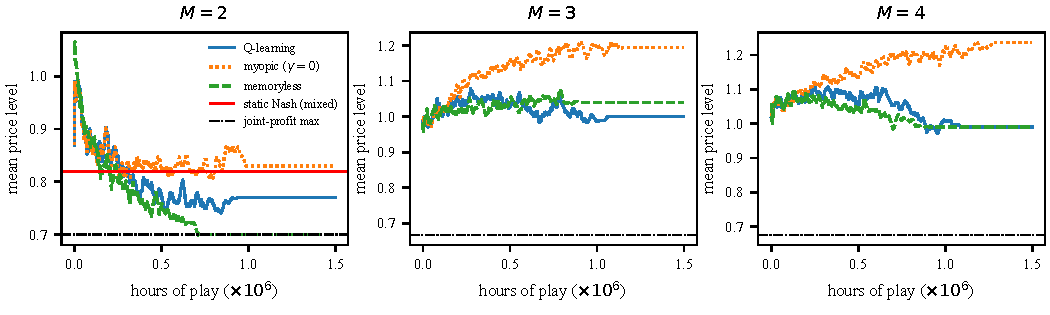
\includegraphics[width=\linewidth]{figs/qlearning.pdf}
\caption{Mean price level while learning (10 seeds), for $M=2,3,4$, against the static Nash and joint-profit benchmarks.}
\label{fig:q}
\end{figure}

\textbf{RQ1: inflated reports (Fig.~\ref{fig:lie}).} These runs use rival-offer learning and $B=300$, and compare against the same seeds with truthful users.
\begin{itemize}
\item With 50\% strategic users ($\delta=0.5$):
  \begin{itemize}
  \item platform spending rises 5.1\%, 4.2\% and 4.1\% for $M=2,3,4$;
  \item profit falls 6.9\%, 10.2\% and 11.6\%;
  \item coverage falls by about 4\%, because higher bounties on contested cells consume budget.
  \end{itemize}
  The direction was the same in all 10 seeds for every $M$.
\item With $M=2$ and 50\% strategic users, the always-honest non-loyal cohort gains 11.3\% (24.4 units per user over the three measured weeks), compared with 12.8\% (28.2 units) for the nested liar cohort used in Fig.~\ref{fig:lie}. The honest cohort's absolute gain is about 14\% smaller. In the matched all-truthful runs the cohorts already had slightly different mean earnings (214.9 versus 218.0 units), despite random assignment among non-loyal users. The difference in cohort gains is not the causal payoff from a unilateral lie.
\item \emph{Sensitivity:}
  \begin{itemize}
  \item with $M=2$ and 50\% strategic users, a larger lie ($\delta=1$) raises the profit loss from 6.9\% to 9.7\%, relative to truthful reporting;
  \item the PACMAB-inspired max update spends more than the moving-average update even with truthful users (331 versus 314 per hour for $M=2$).
  \end{itemize}
\end{itemize}

\begin{figure}[!htbp]\centering
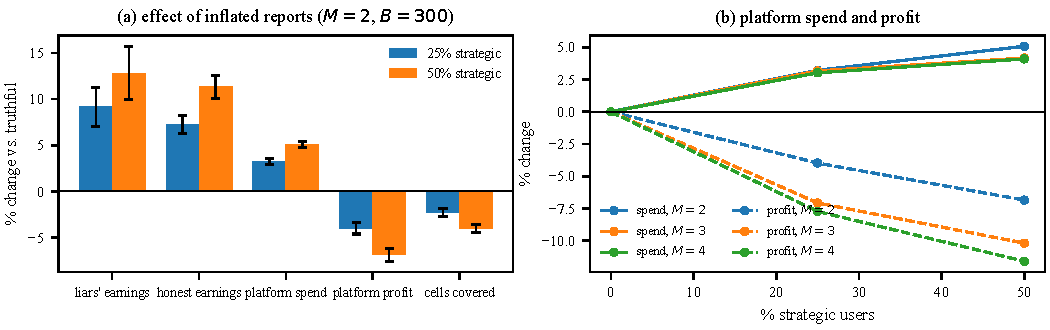
\includegraphics[width=\linewidth]{figs/lying.pdf}
\caption{Effect of inflated rival-offer reports. (a) Percentage change for the same users and seeds against the truthful run ($M=2$; mean $\pm$ s.d.). The liar cohort is the nested 25\% group in both treatments, and the honest cohort consists of non-loyal users truthful in both. (b) Platform spending and profit against the share of strategic users.}
\label{fig:lie}
\end{figure}

\textbf{RQ3 and RQ4: coverage bonus and method comparison (Fig.~\ref{fig:bonus}).}
\begin{itemize}
\item \emph{RQ3.} Each platform reserves 25\% of its budget for low-traffic cells, at equal total budget.
  \begin{itemize}
  \item A $+50\%$ bonus raises low-traffic coverage from 0.74 to 13.6 cells per hour (18-fold), for a 3\% loss in total coverage. This is the premium of Proposition~\ref{prop:cov} in action.
  \item Larger bonuses do worse (7.4 cells at $+300\%$): with a fixed reserve, each bonus task costs more, so fewer can be posted.
  \end{itemize}
\item \emph{RQ4} (equal budgets, truthful users).
  \begin{itemize}
  \item Q-learning covers the most cells per unit spent for every $M$ (31.0 against 22.7 for fixed pricing with $M=2$).
  \item It does so by paying users 43\% less, and the earnings Gini rises from 0.37 to 0.45.
  \item Rival-offer learning is least efficient for $M\ge3$, because of the outbid escalation.
  \end{itemize}
\end{itemize}

\begin{figure}[!htbp]\centering
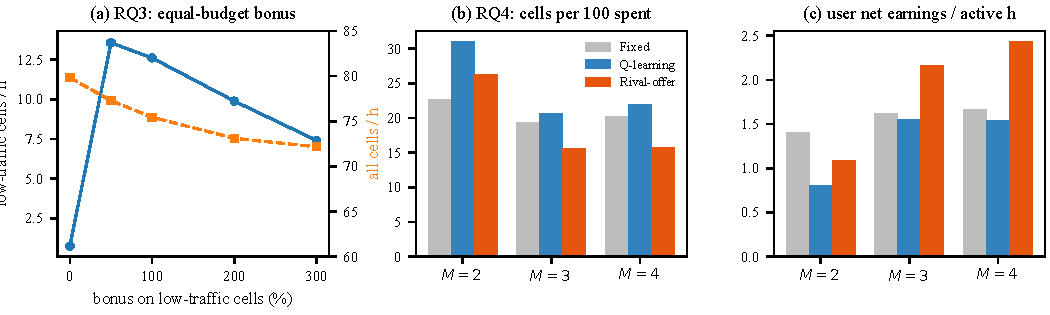
\includegraphics[width=\linewidth]{figs/bonus_methods.pdf}
\caption{(a) Low-traffic and total coverage against the bonus (25\% of budget reserved). (b) Cells covered per 100 units spent, and (c) user earnings, for the three pricing methods at equal budgets.}
\label{fig:bonus}
\end{figure}

\subsection{Insights and next steps}
\textbf{Insights.}
\begin{enumerate}
\item The users' side is a well-behaved potential game. Equilibria are reached in a few sweeps and are near-efficient on real data. The interesting strategic behaviour is therefore on the platforms' side and in the reports.
\item With binding budgets, the price level trades participation against the number of posted tasks. Raising pay or budget barely changes low-traffic coverage, while a targeted bonus raises it substantially.
\item Report-based learning does not guarantee truthful reporting in repeated play. In our runs, inflation cuts platform profit and raises earnings for honest as well as strategic cohorts.
\item Learned pay falls below the competitive benchmark, even without price memory. The control cannot tell us whether forward-looking learners punish deviations.
\end{enumerate}

\textbf{Next steps.}
\begin{enumerate}
\item Implement PACMAB faithfully (UCB with perceptions, personalised offers) for RQ1.
\item Let users learn $\delta$ with a bandit, to see whether lying spreads or dies out.
\item Test simple defences against false reports (trimming, capping, spot checks).
\item Add MSensing and deferred acceptance to RQ4.
\item Run a punishment (impulse-response) test on the real-data Q-learners.
\end{enumerate}

\begin{thebibliography}{99}
\bibitem{yang2012crowdsourcing} D.~Yang, G.~Xue, X.~Fang, and J.~Tang, ``Crowdsourcing to smartphones: Incentive mechanism design for mobile phone sensing,'' in \emph{Proc. ACM MobiCom}, 2012, pp.~173--184.
\bibitem{li2021mp} Y.~Li, F.~Li, S.~Yang, Y.~Wu, H.~Chen, K.~Sharif, and Y.~Wang, ``MP-Coopetition: Competitive and cooperative mechanism for multiple platforms in mobile crowd sensing,'' \emph{IEEE Trans. Serv. Comput.}, vol.~14, no.~6, pp.~1864--1876, 2021.
\bibitem{dongare2026pacmab} S.~J. Dongare, C.~K. Thomas, A.~Ortiz, W.~Saad, and A.~Klein, ``Dynamic hypergame for task assignment in multi-platform mobile crowdsensing under incomplete information,'' arXiv:2605.03569, 2026.
\bibitem{rosenthal1973} R.~W. Rosenthal, ``A class of games possessing pure-strategy Nash equilibria,'' \emph{Int. J. Game Theory}, vol.~2, pp.~65--67, 1973.
\bibitem{monderer1996potential} D.~Monderer and L.~S. Shapley, ``Potential games,'' \emph{Games Econ. Behav.}, vol.~14, no.~1, pp.~124--143, 1996.
\bibitem{blume1993} L.~E. Blume, ``The statistical mechanics of strategic interaction,'' \emph{Games Econ. Behav.}, vol.~5, no.~3, pp.~387--424, 1993.
\bibitem{marden2012revisiting} J.~R. Marden and J.~S. Shamma, ``Revisiting log-linear learning: Asynchrony, completeness and payoff-based implementation,'' \emph{Games Econ. Behav.}, vol.~75, no.~2, pp.~788--808, 2012.
\bibitem{vetta2002} A.~Vetta, ``Nash equilibria in competitive societies, with applications to facility location, traffic routing and auctions,'' in \emph{Proc. IEEE FOCS}, 2002, pp.~416--425.
\bibitem{watkins1992} C.~J. C.~H. Watkins and P.~Dayan, ``Q-learning,'' \emph{Mach. Learn.}, vol.~8, pp.~279--292, 1992.
\bibitem{calvano2020ai} E.~Calvano, G.~Calzolari, V.~Denicol\`o, and S.~Pastorello, ``Artificial intelligence, algorithmic pricing, and collusion,'' \emph{Amer. Econ. Rev.}, vol.~110, no.~10, pp.~3267--3297, 2020.
\bibitem{fiandrino2017crowdsensim} C.~Fiandrino, A.~Capponi, G.~Cacciatore, D.~Kliazovich, U.~Sorger, P.~Bouvry, B.~Kantarci, F.~Granelli, and S.~Giordano, ``CrowdSenSim: A simulation platform for mobile crowdsensing in realistic urban environments,'' \emph{IEEE Access}, vol.~5, pp.~3490--3503, 2017.
\bibitem{yuan2010tdrive} J.~Yuan, Y.~Zheng, C.~Zhang, W.~Xie, X.~Xie, G.~Sun, and Y.~Huang, ``T-Drive: Driving directions based on taxi trajectories,'' in \emph{Proc. ACM SIGSPATIAL GIS}, 2010, pp.~99--108.
\bibitem{zheng2010geolife} Y.~Zheng, X.~Xie, and W.-Y. Ma, ``GeoLife: A collaborative social networking service among user, location and trajectory,'' \emph{IEEE Data Eng. Bull.}, vol.~33, no.~2, pp.~32--39, 2010.
\bibitem{kazil2020mesa} J.~Kazil, D.~Masad, and A.~Crooks, ``Utilizing Python for agent-based modeling: The Mesa framework,'' in \emph{Proc. SBP-BRiMS}, 2020, pp.~308--317.
\end{thebibliography}
\end{document}
